\documentclass{beamer}
\usepackage[utf8]{inputenc}
\usetheme{Madrid}
\usecolortheme{default}
\usepackage{amsmath,amssymb,amsfonts,amsthm}
\usepackage{txfonts}
\usepackage{tkz-euclide}
\usepackage{listings}
\usepackage{adjustbox}
\usepackage{array}
\usepackage{tabularx}
\usepackage{gvv}
\usepackage{lmodern}
\usepackage{circuitikz}
\usepackage{tikz}
\usepackage{graphicx}
\setbeamertemplate{page number in head/foot}[totalframenumber]
\usepackage{tcolorbox}
\tcbuselibrary{minted,breakable,xparse,skins}
\definecolor{bg}{gray}{0.95}
\DeclareTCBListing{mintedbox}{O{}m!O{}}{%
breakable=true,
listing engine=minted,
listing only,
minted language=#2,
minted style=default,
minted options={%
linenos,
gobble=0,
breaklines=true,
breakafter=,,
fontsize=\small,
numbersep=8pt,
#1},
boxsep=0pt,
left skip=0pt,
right skip=0pt,
left=25pt,
right=0pt,
top=3pt,
bottom=3pt,
arc=5pt,
leftrule=0pt,
rightrule=0pt,
bottomrule=2pt,
toprule=2pt,
colback=bg,
colframe=orange!70,
enhanced,
overlay={%
\begin{tcbclipinterior}
\fill[orange!20!white] (frame.south west) rectangle ([xshift=20pt]frame.north west);
\end{tcbclipinterior}},
#3,
}
\lstset{
language=C,
basicstyle=\ttfamily\small,
keywordstyle=\color{blue},
stringstyle=\color{orange},
commentstyle=\color{green!60!black},
numbers=left,
numberstyle=\tiny\color{gray},
breaklines=true,
showstringspaces=false,
}

\title
{5.8.40}
\date{October 3, 2025}
\author
{EE25BTECH11043 - Nishid Khandagre}

\begin{document}

\frame{\titlepage}

\begin{frame}{Question}
The ratio of incomes of two persons is 9:7 and the ratio of their expenditures is 4:3. If each of them manages to save rupees 2000 per month, find their monthly incomes.
\end{frame}

\begin{frame}{Solution}
Let the monthly incomes be $x$ and $y$.

Given ratio of their incomes:
    \begin{align}
    \frac{x}{y} &= \frac{9}{7} \\
    7x - 9y &= 0
    \end{align}

Expenditures are Income $-$ Savings.
Expenditures of the two persons are $x-2000$ and $y-2000$.\\
Given expenditure ratio:
    \begin{align}
    \frac{x-2000}{y-2000} &= \frac{4}{3} \\
    3x - 6000 &= 4y - 8000 \\
    3x - 4y &= -2000
    \end{align}
\end{frame}

\begin{frame}{Solution}
\begin{align}
7x - 9y &= 0 \\
3x - 4y &= -2000
\end{align}
Matrix form:
\begin{align}
\myvec{7 & -9 \\ 3 & -4}
\myvec{x \\ y}
=
\myvec{0 \\ -2000}
\end{align}
Augmented matrix:
\begin{align}
\myaugvec{2}
{
7 & -9 & 0 \\
3 & -4 & -2000 \\
}
\end{align}
\end{frame}

\begin{frame}{Solution}

Then $R_2 \rightarrow 7R_2 - 3R_1$:
\begin{align}
\myaugvec{2}{
7 & -9 & 0 \\
0 & -1 & -14000
}
\end{align}
Then $R_2 \rightarrow -R_2$:
\begin{align}
\myaugvec{2}{
 7 & -9 & 0 \\
 0 & 1 & 14000
}
\end{align}

Then $R_1 \rightarrow R_1 + 9R_2$:
\begin{align}
\myaugvec{2}{
7 & 0 & 126000 \\
0 & 1 & 14000
}
\end{align}
Then $R_1 \rightarrow \frac{1}{7}R_1$:
\begin{align}
\myaugvec{2}{
1 & 0 & 18000 \\
0 & 1 & 14000
}
\end{align}
\end{frame}

\begin{frame}{Solution}
\begin{align}
\myvec{x\\y}&=\myvec{18000\\14000}
\end{align}

\begin{align}
x &= \rupee{18000} \\
y &= \rupee{14000}
\end{align}
The monthly incomes are \rupee{18000} and \rupee{14000}.
\end{frame}

\begin{frame}[fragile]
\frametitle{C Code}
\begin{lstlisting}
#include <stdio.h>

// Function to solve a 2x2 system of linear equations using Cramer's Rule
// a1*x + b1*y = c1
// a2*x + b2*y = c2
//   a1, b1, c1: Coefficients and constant for the first equation
//   a2, b2, c2: Coefficients and constant for the second equation
//   *x_solution: Pointer to store the solution for x
//   *y_solution: Pointer to store the solution for y
int solve_2x2_system(double a1, double b1, double c1,
                      double a2, double b2, double c2,
                      double *x_solution, double *y_solution) {

    double determinant = a1 * b2 - a2 * b1;
\end{lstlisting}
\end{frame}

\begin{frame}[fragile]
\frametitle{C Code}
\begin{lstlisting}
    // Check if a unique solution exists
    if (determinant == 0) {
        // No unique solution (parallel lines or same line)
        return 0;
    }

    double det_x = c1 * b2 - c2 * b1;
    double det_y = a1 * c2 - a2 * c1;

    *x_solution = det_x / determinant;
    *y_solution = det_y / determinant;

    return 1; // Unique solution found
}
\end{lstlisting}
\end{frame}

\begin{frame}[fragile]
\frametitle{Python Code using C shared library}
\begin{lstlisting}
import ctypes
import numpy as np
import matplotlib.pyplot as plt
# Load the shared library
lib_solver = ctypes.CDLL("./code12.so")

# Define the argument types and return type for the C function
# int solve_2x2_system(double a1, double b1, double c1,
#                      double a2, double b2, double c2,
#                      double *x_solution, double *y_solution)
lib_solver.solve_2x2_system.argtypes = [
    ctypes.c_double, ctypes.c_double, ctypes.c_double,  # a1, b1, c1
    ctypes.c_double, ctypes.c_double, ctypes.c_double,  # a2, b2, c2
    ctypes.POINTER(ctypes.c_double),                     # x_solution
    ctypes.POINTER(ctypes.c_double)                      # y_solution
]
\end{lstlisting}
\end{frame}

\begin{frame}[fragile]
\frametitle{Python Code using C shared library}
\begin{lstlisting}
lib_solver.solve_2x2_system.restype = ctypes.c_int

# --- Problem: Income and Expenditure ---
# Equations:
# 1) 9x - 4y = 2000
# 2) 7x - 3y = 2000

# Coefficients for the C solver
a1, b1, c1 = 9.0, -4.0, 2000.0
a2, b2, c2 = 7.0, -3.0, 2000.0

# Create ctypes doubles to hold the results for x and y multipliers
x_multiplier_result = ctypes.c_double()
y_multiplier_result = ctypes.c_double()
\end{lstlisting}
\end{frame}

\begin{frame}[fragile]
\frametitle{Python Code using C shared library}
\begin{lstlisting}
# Call the C function to solve the system
print("Solving the system of equations for income and expenditure multipliers using C function:")
print(f"  Equation 1: {a1}x + {b1}y = {c1}")
print(f"  Equation 2: {a2}x + {b2}y = {c2}")

success = lib_solver.solve_2x2_system(
    a1, b1, c1,
    a2, b2, c2,
    ctypes.byref(x_multiplier_result),
    ctypes.byref(y_multiplier_result)
)

if success:
    x_solution = x_multiplier_result.value
    y_solution = y_multiplier_result.value
\end{lstlisting}
\end{frame}

\begin{frame}[fragile]
\frametitle{Python Code using C shared library}
\begin{lstlisting}
    print(f"\nSolution found (intersection point):")
    print(f"  x (income multiplier) = {x_solution:.2f}")
    print(f"  y (expenditure multiplier) = {y_solution:.2f}")

    # --- Plotting the two lines and their intersection ---
    plt.figure(figsize=(10, 8))

    # Generate points for the lines
    # We'll use a range around the solution to make the intersection clear
    x_vals_range = np.linspace(x_solution - 1000, x_solution + 1000, 400) # Extend range for visualization
\end{lstlisting}
\end{frame}

\begin{frame}[fragile]
\frametitle{Python Code using C shared library}
\begin{lstlisting}
    # Plotting Eq 1: a1*x + b1*y = c1  => y = (c1 - a1*x) / b1
    if b1 != 0:
        y1_vals = (c1 - a1 * x_vals_range) / b1
        plt.plot(x_vals_range, y1_vals, label=f'{a1:.0f}x + {b1:.0f}y = {c1:.0f} (Eq 1)', color='blue')
    elif a1 != 0: # Handle vertical line case: x = c1/a1
        plt.axvline(x=c1/a1, label=f'x = {c1/a1:.0f} (Eq 1)', color='blue', linestyle='--')
    else:
        print("Equation 1 is trivial (0=C). Not plotted.")
    # Plotting Eq 2: a2*x + b2*y = c2  => y = (c2 - a2*x) / b2
    if b2 != 0:
        y2_vals = (c2 - a2 * x_vals_range) / b2
        plt.plot(x_vals_range, y2_vals, label=f'{a2:.0f}x + {b2:.0f}y = {c2:.0f} (Eq 2)', color='red')
    elif a2 != 0: # Handle vertical line case: x = c2/a2
        plt.axvline(x=c2/a1, label=f'x = {c2/a2:.0f} (Eq 2)', color='red', linestyle='--')
        \end{lstlisting}
\end{frame}

\begin{frame}[fragile]
\frametitle{Python Code using C shared library}
\begin{lstlisting}
    else:
        print("Equation 2 is trivial (0=C). Not plotted.")

    # Plot the intersection point
    plt.scatter(x_solution, y_solution, color='green', s=150, zorder=5,
                label=f'Intersection ({x_solution:.0f}, {y_solution:.0f})')
    plt.annotate(f'({x_solution:.0f}, {y_solution:.0f})',
                 (x_solution, y_solution), textcoords="offset points", xytext=(5,5), ha='left',
                 bbox=dict(boxstyle="round,pad=0.3", fc="yellow", ec="b", lw=1, alpha=0.7))

    plt.xlabel('Income Multiplier (x)')
    \end{lstlisting}
\end{frame}

\begin{frame}[fragile]
\frametitle{Python Code using C shared library}
\begin{lstlisting}
    plt.ylabel('Expenditure Multiplier (y)')
    plt.title('Graphical Solution of Income and Expenditure Equations')
    plt.grid(True)
    plt.legend()
    plt.gca().set_aspect('auto', adjustable='box')
    plt.xlim(min(x_vals_range), max(x_vals_range))
    plt.ylim(min(y1_vals.min(), y2_vals.min(), y_solution) - 500, max(y1_vals.max(), y2_vals.max(), y_solution) + 500)
    plt.show()

else:
    print("\nError: No unique solution exists for this system (determinant is zero).")
    print("The lines are either parallel or the same line, which should not happen for this problem.")
\end{lstlisting}
\end{frame}

\begin{frame}[fragile]
\frametitle{Direct Python Code }
\begin{lstlisting}
import numpy as np
import numpy.linalg as LA
import matplotlib.pyplot as plt

# --- Problem: Income and Expenditure ---
# The ratio of incomes of two persons is 9:7 => Incomes: 9x, 7x
# The ratio of their expenditures is 4:3   => Expenditures: 4y, 3y
# Each saves 2000 per month.
#
# Equations:
# 1) Income1 - Expenditure1 = Savings  => 9x - 4y = 2000
# 2) Income2 - Expenditure2 = Savings  => 7x - 3y = 2000

# Represent the system as Ax = B
# A = [[9, -4],
#      [7, -3]]
# x = [x_multiplier, y_multiplier]
# B = [2000, 2000]
\end{lstlisting}
\end{frame}

\begin{frame}[fragile]
\frametitle{Direct Python Code }
\begin{lstlisting}
A_matrix = np.array([[9.0, -4.0],
                 [7.0, -3.0]])

B_vector = np.array([2000.0, 2000.0])

print("Solving the system of equations for income and expenditure multipliers:")
print(f"  Equation 1: {A_matrix[0,0]}x + {A_matrix[0,1]}y = {B_vector[0]}")
print(f"  Equation 2: {A_matrix[1,0]}x + {A_matrix[1,1]}y = {B_vector[1]}")

 # Solve the system of linear equations using numpy.linalg.solve
solution = LA.solve(A_matrix, B_vector)
x_solution = solution[0]
y_solution = solution[1]
\end{lstlisting}
\end{frame}

\begin{frame}[fragile]
\frametitle{Direct Python Code }
\begin{lstlisting}
print(f"  x (income multiplier) = {x_solution:.2f}")
print(f"  y (expenditure multiplier) = {y_solution:.2f}")
   # --- Plotting the two lines and their intersection ---
plt.figure(figsize=(10, 8))

# Define a generous range for x_vals for plotting purposes.
# Knowing the solution (x=2000, y=4000), we can set a reasonable range.
x_plot_min = x_solution - 1000
x_plot_max = x_solution + 1000
x_vals_range = np.linspace(x_plot_min, x_plot_max, 400)

# Plotting Equation 1: a1*x + b1*y = c1  => y = (c1 - a1*x) / b1
# Coefficients from A_matrix and B_vector
y1_vals = (B_vector[0] - A_matrix[0,0] * x_vals_range) / A_matrix[0,1]
plt.plot(x_vals_range, y1_vals, "b-", label=f'{A_matrix[0,0]:.0f}x {A_matrix[0,1]:+.0f}y = {B_vector[0]:.0f} (Person 1)')
\end{lstlisting}
\end{frame}

\begin{frame}[fragile]
\frametitle{Direct Python Code }
\begin{lstlisting}
# Plotting Equation 2: a2*x + b2*y = c2  => y = (c2 - a2*x) / b2
y2_vals = (B_vector[1] - A_matrix[1,0] * x_vals_range) / A_matrix[1,1]
plt.plot(x_vals_range, y2_vals, "r-", label=f'{A_matrix[1,0]:.0f}x {A_matrix[1,1]:+.0f}y = {B_vector[1]:.0f} (Person 2)')

 # Plot the intersection point
plt.scatter(x_solution, y_solution, color='green', s=150, zorder=5,
            label=f'Intersection ({x_solution:.0f}, {y_solution:.0f})')
plt.annotate(f'({x_solution:.0f}, {y_solution:.0f})',
             (x_solution, y_solution), textcoords="offset points", xytext=(5,5), ha='left',
             bbox=dict(boxstyle="round,pad=0.3", fc="yellow", ec="b", lw=1, alpha=0.7))
\end{lstlisting}
\end{frame}

\begin{frame}[fragile]
\frametitle{Direct Python Code }
\begin{lstlisting}
plt.xlabel('Income Multiplier (x)')
plt.ylabel('Expenditure Multiplier (y)')
plt.title('Graphical Solution of Income and Expenditure Equations')
plt.grid(True)
plt.legend(loc='best')

# Set plot limits based on data for good visualization
y_plot_min = min(y1_vals.min(), y2_vals.min(), y_solution) - 500
y_plot_max = max(y1_vals.max(), y2_vals.max(), y_solution) + 500
plt.xlim(x_plot_min, x_plot_max)
plt.ylim(y_plot_min, y_plot_max)
plt.gca().set_aspect('auto', adjustable='box')

plt.savefig("fig2.png")
plt.show()

print("Figure saved as fig2.png")
\end{lstlisting}
\end{frame}

\begin{frame}{Plot by Python using shared output from C}
\begin{figure}[H]
\centering
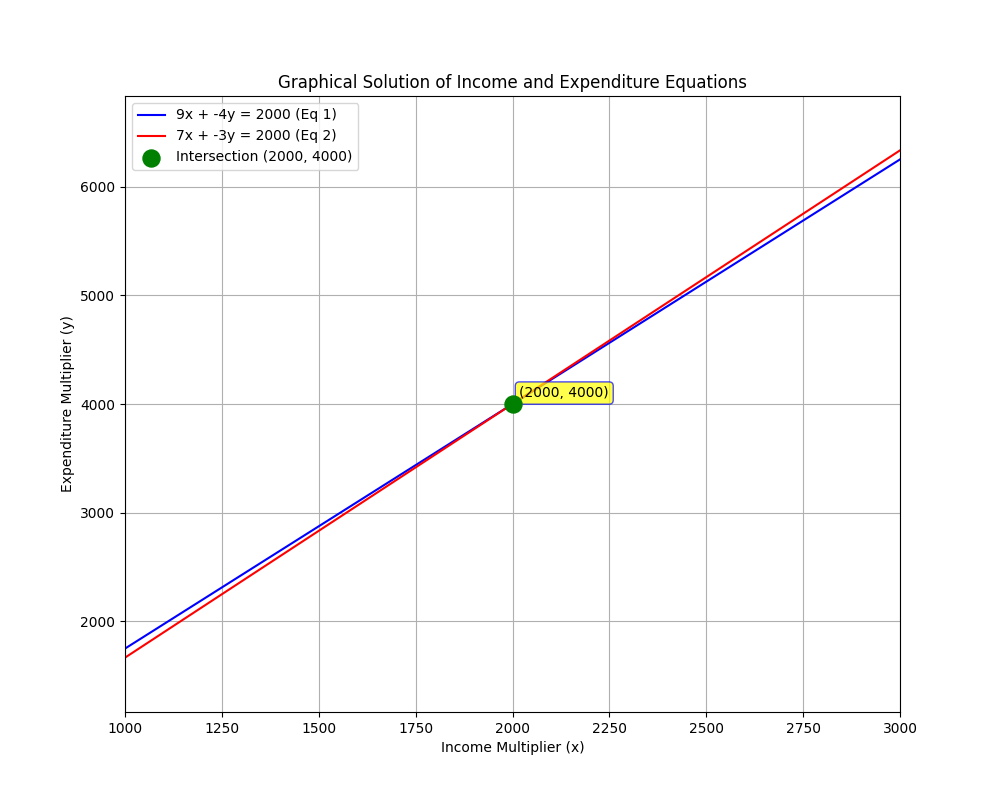
\includegraphics[width=0.8\columnwidth]{../figs/fig1.png}
\caption{}
\label{fig:1}
\end{figure}
\end{frame}

\begin{frame}{Plot by Python only}
\begin{figure}[H]
\centering
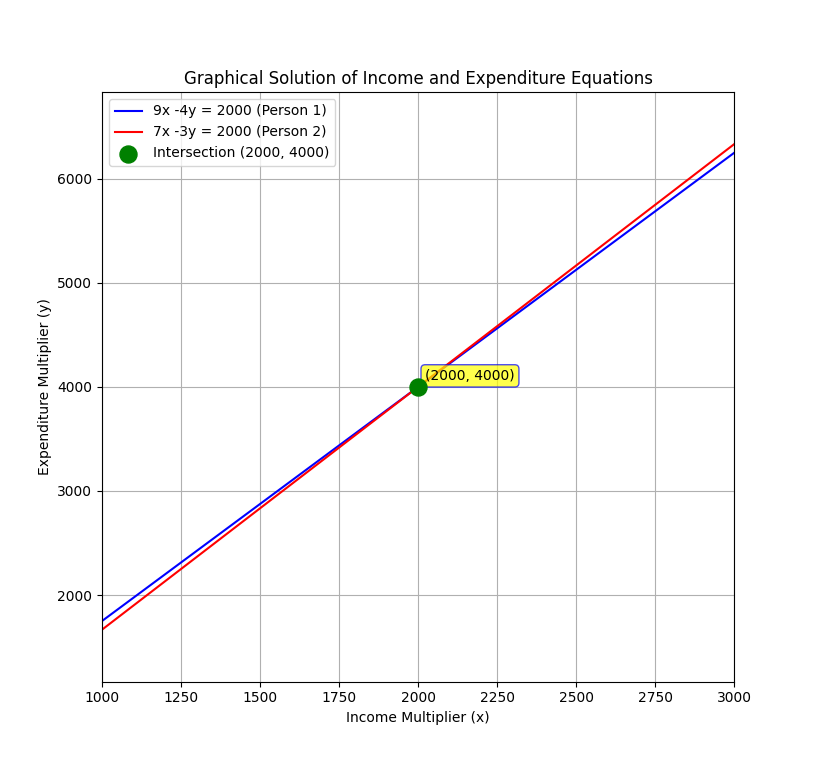
\includegraphics[width=0.7\columnwidth]{../figs/fig2.png}
\caption{}
\label{fig:2}
\end{figure}
\end{frame}

\end{document}
